% -----------------------------------------------
% Template for ISMIR Papers
% 2016 version, based on previous ISMIR templates

% Requirements :
% * 6+1 page length maximum
% * 2MB maximum file size
% * Copyright note must appear in the bottom left corner of first page
% (see conference website for additional details)
% -----------------------------------------------

\documentclass{article}
\usepackage{ismir,amsmath,cite}
\usepackage{graphicx}
\usepackage{color}
\usepackage{booktabs}

\usepackage{array}
\newcolumntype{L}[1]{>{\raggedright\let\newline\\\arraybackslash\hspace{0pt}}m{#1}}
\newcolumntype{C}[1]{>{\centering\let\newline\\\arraybackslash\hspace{0pt}}m{#1}}
\newcolumntype{R}[1]{>{\raggedleft\let\newline\\\arraybackslash\hspace{0pt}}m{#1}}

% Title.
% ------
\title{Music Transcription with Multilabel Classification}

% Note: Please do NOT use \thanks or a \footnote in any of the author markup

% Single address
% To use with only one author or several with the same address
% ---------------
%\oneauthor
% {Names should be omitted for double-blind reviewing}
% {Affiliations should be omitted for double-blind reviewing}

% Two addresses
% --------------
%\twoauthors
%  {First author} {School \\ Department}
%  {Second author} {Company \\ Address}

%% To make customize author list in Creative Common license, uncomment and customize the next line
%  \def\authorname{First Author, Second Author} 


% Three addresses
% --------------
\threeauthors
  {Nora Huang} {Department of Computer Science\\
University of Victoria\\
Victoria, B.C, Canada \\ {\tt norah@uvic.ca}}
  {Aazim Lakhani} {Department of Computer Science\\
University of Victoria\\
Victoria, B.C, Canada \\ {\tt aazimlakhani@uvic.ca}}
  {Parul Parul} {Department of Computer Science\\
University of Victoria\\
Victoria, B.C, Canada \\ {\tt pparul@uvic.ca}}

%% To make customize author list in Creative Common license, uncomment and customize the next line
%  \def\authorname{First Author, Second Author, Third Author} 

% Four or more addresses
% OR alternative format for large number of co-authors
% ------------
%\multauthor
%{First author$^1$ \hspace{1cm} Second author$^1$ \hspace{1cm} Third author$^2$} { \bfseries{Fourth author$^3$ \hspace{1cm} Fifth author$^2$ \hspace{1cm} Sixth author$^1$}\\
%  $^1$ Department of Computer Science, University , Country\\
%$^2$ International Laboratories, City, Country\\
%$^3$  Company, Address\\
%{\tt\small CorrespondenceAuthor@ismir.edu, PossibleOtherAuthor@ismir.edu}
%}
%\def\authorname{First author, Second author, Third author, Fourth author, Fifth author, Sixth author}


\sloppy % please retain sloppy command for improved formatting

\begin{document}

%
\maketitle
%
\begin{abstract}
Automatic music transcription is an active research topic in the field of Music Information Retrieval (MIR). The goal of music transcription is to determine the score-like representation of the input audio music. The technologies of it have been used in many mobile and web applications. However, the accuracy of the current transcription approach is still below that of a human expert. The majority of current research is focused on how to separate the pitches from the audio, then estimate them. In this project, time and frequency domain features for piano music files were extracted. The data was filtered through normalization, and feature subsets with maximum entropy and correlation were selected for use in well known classifiers such as Decision Trees, Random Tree, Nearest Neighbor, and SVM. This process enables the project model to detect musical notes which could be used in automatic music transcription.
\end{abstract}
%
\section{Introduction}\label{sec:introduction}
Automatic music transcription is the process of translating an audio music signal into a musical score sheet\cite{Duan2015-nt}. There are many applications of this technology, such as helping a student learn how to play music for well known soundtracks using a specific instrument. It could do so by building playable score sheets they could use for practice. It could also allow a musician or composer to record their improvised performance\cite{Benetos2013-io} and share their work for others to reproduce. There are various approaches to achieve these goals\cite{Ming2014-cj,Lee2012-dd,Anan2012-up,Sigtia2016-sz,Poliner2005-ow}. 

An ideal piece of music for transcription has clear, simple, and easily differentiable sounds. However in reality, song compositions are complex pieces of work with many different instruments and human voices. Addressing this complexity is a significant challenge. This project focuses on the problem of monophonic and polyphonic piano music for up to 4 notes. Monophonic includes a single melodic line with no accompaniment, while polyphonic may have multiple melodic lines mostly independent or in imitation of one another. In other words, this project focuses exclusively on music composed with up to 4 notes played simultaneously.

This project builds a unique model to recognize keys used to played music notes to support music transcription. First, windows are applied to the input music files to segment the audio into frames around 11ms in length. In total, it retrieves 512 digital samples per frame. In total, 63 features are extracted from each frame. These acoustic features are post-processed by removing silent frames or values and labelling each non-silent frame, then analysed with either Weka\cite{Holmes1994-kg} and Meka\cite{Read2012-sh} to reduce the set into several reasonably sized feature subsets.  The selected features are those having high entropy or co-relation, which are then passed through well known classifiers to prepare a model. 

Weka is used to analyse monophonic music which can simplified as the single-label classification problem. Conversely, Meka is a multi-label classification extension of Weka to  analyse polyphonic music, equivalent to a multilabel classification problem. Polyphonic music exposes the challenge of detecting the right keys used to play a chord when several others notes from potentially many different instruments are played simultaneously. This project reduces the scope of the problem by focusing on single-instrument audio tracks, leaving only the problem of detecting each note in a chord. In total, Multilabel classification\cite{Herrera2016-ep} is applied using 4 classifiers: IBK\cite{Aha1991-ir}, J48\cite{Ross_Quinlan2014-rg}, SMO\cite{Platt1999-iq}, and RandomTree\cite{Dugan2015-fn}. 

The overview of the project model is described in Figure \ref{figure1}. The classifiers are trained and tested based on this model.

\begin{figure}[h]
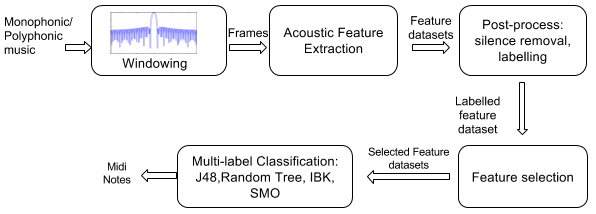
\includegraphics[scale=.4]{overview}
 \caption{System Flow Diagram}
\label{figure1}
\end{figure}

The structure of the report is as follows: first, the dataset for the project is described. The tool and methods used for feature extraction are then described, along with the meaning of each set of features. Next, feature selection describes how the feature subsets were derived, analysed, and grouped. The classification section details the classifiers used and the parameters of each for every feature subset, including details on how they were trained and tested. The results of all the experiments are then evaluated and visualized for each dataset. Finally, the results are concluded and future work is outlined.

 
%
\section{Dataset}\label{sec:Dataset}
The model described in Section 1, Figure\ref{figure1} is evaluated using the MIDI (Musical Instrument Digital Interface)  Aligned Piano Sounds (MAPS) dataset\cite{Emiya2010-ki}. Due to copyright licensing, there are a limited number of datasets available for research. MAPS is a widely used piano database for multipitch estimation and automatic transcription of music. It provides recordings with CD quality (16-bit , 44 kHz sampled stereo audio) sounds. It is freely available under the Creative Commons License. It consists of audio files with corresponding annotations for isolated sounds, chords, and complete pieces of piano music under various different recording conditions, including various closed rooms and close ambient takes. MAPS can be divided into 4 sets: \\\\
ISOL (isolated notes and musical excerpts)\\
RAND (Chords with random pitch notes.)\\
UCHO (Usual chords from Western music)\\
MUS (Pieces of piano music)\\\\
For monophonic music, we use 2 second notes from the ISOL dataset. This is defined as P1 for the remainder of this report. For polyphonic music, we use polyphonic sounds with 2 to 4 notes from the RAND set. They are similarly defined as P2, P3, and P4 for the remainder of this report.
\section{Feature Extraction}\label{sec:features}
In the signal processing domain, feature extraction is one of the most widely used methods to analyse a signal. There are several parts to one audio signal offering varying amounts of useful information. This section explores some of these features and selects some for use based on how much they contribute to the goal of automatic music transcription.
\subsection{Feature Extraction Tool}
Marsyas (Music Analysis, Retrieval and Synthesis for Audio Signals) is an open source software framework for audio processing with specific emphasis on MIR applications \cite{Tzanetakis2000-xp}. Bextract is one of the most powerful executables provided by Marsyas. It can be used for complete feature extraction and classification experiments with multiple files. However its classification feature is limited and did not fulfill the requirement of this project. As such, only the feature extraction functionality is used.
\subsection{Feature Extraction Strategy}
Using Bextract provided, the features for each frame are extracted. By default, the frame size of Bextract is 512 samples which matches the dataset sampled from MAPS. In total, it extracts 63 features from each frame. The results are formatted and stored in .arff format file for later processing. Bextract further handles the labeling for each item by using a single label - it does not support multi-labelling. As such, for the polyphonic music requiring multi-labeling, they are manually labeled with multiple values corresponding to the notes it consists of. This is done by post-processed the output .arff files with a script uniquely created for this project. This enables the data to be run directly on Meka. The script derives the labels for the output from the corresponding .txt annotations provided with the sound from MAPS. 
\subsection{Acoustic Features}
From each frame, 63 acoustic features were extracted. They are combinations of the following 5 parameters:\\
\textbf{Time-domain Zero-Crossings}  is the point where the sign of a mathematical function changes (e.g.,  from positive to negative), represented by a crossing of the axis (zero value) in the graph of the function\cite{Bundy1984-fo}. It is a commonly used term in electronics, mathematics, sound, and image processing.\\
\textbf{Spectral Centroid} is a measure used in digital signal processing to characterise a spectrum. It indicates where the "center of mass" of the spectrum is. Perceptually, it has a robust connection with the impression of "brightness" of a sound.\\
\textbf{Rolloff} is the steepness of a transmission function with frequency.\\
\textbf{Flux} is a measure of how quickly the power spectrum of a signal is changing, calculated by comparing the power spectrum for one frame against the power spectrum from the previous frame. More precisely, it is usually calculated as the 2-norm (also known as the Euclidean distance) between the two normalised spectra.\\
\textbf{Mel-Frequency Cepstral Coefficients} are coefficients that collectively make up an  mel-frequency cepstrum (MFC). In sound processing, the MFC is a representation of the short-term power spectrum of a sound, based on a linear cosine transform of a log power spectrum on a nonlinear mel scale of frequency.
\section{Feature Selection}
The feature set produced by Bextract, while effective, is a large feature set making human understanding of the data difficult. Feature selection was needed in order to reduce the usable attribute set from 63 into a more reasonable size. This section outlines the approach and result of feature set selection.
\subsection{Filter-based Selection}
There are multiple techniques that may be used to reduce a feature set, including using domain knowledge of the data to manually reduce it, tailoring the set for a specific classifier, or using a systematic filter-based approach\cite{hall1999correlation}. Due to the complexity of the notes and their acoustic features, and the desire to have a general feature set for use in any classifier, the systematic approach was used to decide which features were most useful.\\
Three approaches were used to create 5 feature sets for each PN dataset: 1) learner, 2) entropy, and 3) pearson correlation coefficient. The accuracy results of each feature set was compared against the original for 4 different classifiers in 5-fold cross validation. In order to create a standardized set selection across the datasets (i.e., they all have the same thresholds and features), the P1 dataset was selected as the baseline. That is, the feature subsets generated for P1 were assumed to be sufficient for P2 - P4.
\subsection{Results}
WEKA’s ‘select attributes’ toolset\cite{hall2003benchmarking} was used to generate data for each approach. Two feature subsets were created from the entropy results; any attribute that provided an information gain greater or equal to 0.05 was used in the first entropy feature data set. A second set was created using a threshold of 0.05. Similarly, the pearson result was split into two feature subset using threshold values of 0.03 and 0.02. The threshold values were chosen by observation as they provided either approximately half the original feature set or slightly less which was agreed to be a reasonable attribute set size. Table\ref{table1} summarizes the results.
\begin{table}[h]
 \begin{center}
  \caption{Feature subset selection attribute size results}
\begin{tabular}{|C{1.5cm}|C{1.5cm}|C{1.5cm}|C{1.5cm}|}
      \hline
         Filter Algorithm & Threshold & Attributes Size & Reduced \% \\
         \hline
        %\midline
       
         None &  N/A& 63   & -- \\
         \hline
         Learner & N/A & 28  & 66  \\
        \hline
        Entropy & 0.05 & 14 & 77  \\
       \cline{2-4}
         & 0.03 & 31 & 51    \\
         \hline
        Pearson & 0.03 & 27 &57     \\
        \cline{2-4}
        & 0.02 & 36 &43     \\
       \hline
        %Note. Values are given as mean $\pm$ SD.   &                      &                     \\
\end{tabular}
\end{center}
 \label{table1}
\end{table}

\section{Preprocessing with Normalization}
Normalization scales all numeric variables in the range [0,1] to ensure the outputs are scale invariant. In other words, it makes sure big values don’t dominate smaller ones. One possible formula is given below:\\\\
$\chi_{new} = \dfrac{\chi-\chi_{min}}{\chi_{max}-\chi_{min}}$\\\\
Normalization was used on the P1 original dataset (i.e., with all 63 attributes) to determine if this technique could improve the accuracy of the results. As seen in Table\ref{table2}, the results of normalization did not significantly improve the accuracy of 4 different classifiers. This result meant that normalization was not applied, and was not attempted for the remaining P2-P4 datasets.
\begin{table}[h]
 \begin{center}
  \caption{Accuracy Results Compare (\%)}
\begin{tabular}{|C{2cm}|C{1cm}|C{1cm}|C{1cm}|C{1.5cm}|}
      \hline
          & IBK & J48  & SMO &Random tree \\
         \hline
        %\midline
       
         Without Normalization & 97.98& 88.98& 54.75   & 87.65 \\
         \hline
         With Normalization & 97.98 & 88.98  & 54.76 &  87.67\\
       \hline
\end{tabular}
\end{center}
 \label{table2}
\end{table}

\section{Multilabel Classification}\label{sec:Classifiers}
In MIR, multi-label classification are usually used to identify genres or emotion recognition, but are not used in transcription. Current research into automatic transcription tends to focus only on either the main melody, or on the approach by separating the multiple melodic lines and processing them individually. This project explores multilabel classification for polyphonic transcription by treating each note from the multiple melodic lines as a label, where each label is one of 88 classes corresponding to 88 piano keys (i.e., 11 octaves of 8 notes).\\
Using the feature attribute subsets derived in Section 4, four classifiers were used to experiment with results on all datasets from P1 to P4. The four classifiers were: 1) IBK, 2) J48, 3) SMO, and 4) RandomTree. Training and testing was executed in 5 fold cross-validation on each dataset. This section presents the raw data results and some visualization of the data.

\section{Evaluation}\label{sec:Evaluation}
This section presents the results of running the training and testing classifiers on the P1 dataset in Weka, and the same approach for P2 - P4 in Meka. All datasets use the feature subsets derived in Section 4, and each dataset is separated into its own subsection. 

\subsection{P1 Monophonic Dataset Evaluation}
This section presents the results of the first dataset, provides visualizations of the J48 tree, and analyses the J48 confusion matrix. J48 was chosen for further analysis as it was quick to reproduce on any machine while not sacrificing accuracy.\\
\textbf{Feature subset results}\\
Table \ref{table3} summarizes the result of each classifier on each feature subset. Anecdotally, SMO took the longest amount of time to run (approximately 5-10 minutes) and was assumed to have the worst performance, validated by it’s low correct percentage classified results. IBK took a moderate amount of time to run while providing the highest accuracy. RandomTree was slightly faster than J48 but produced consistent lower accuracies. 
\begin{table}[h]
 \begin{center}
  \caption{Accuracy results of different feature subsets on different classifiers (\%)}
\begin{tabular}{|C{2cm}|C{1cm}|C{1cm}|C{1cm}|C{1.5cm}|}
      \hline
          Filter (Threshold)& IBK & J48  & SMO &Random tree \\
         \hline
         Original & 97.98 & 88.98 & 54.75 & 87.65\\
         \hline
         Learner  & 97.37 & 88.54 & 46.11 & 87.63\\
          \hline
         Entropy (0.05) & 91.48 & 87.08 & 27.88 & 86.87\\
         \hline
         Entropy (0.03)  & 98.61 & 88.59 & 51.86 & 87.83\\
         \hline
         Pearson (0.03) & 99.41 & 87.27 & 48.96 & 87.26\\
         \hline
         Pearson (0.02)  & 99.14 & 88.10 & 48.58 & 87.86\\
       \hline
\end{tabular}
\end{center}
 \label{table3}
\end{table}
\begin{figure}[h]
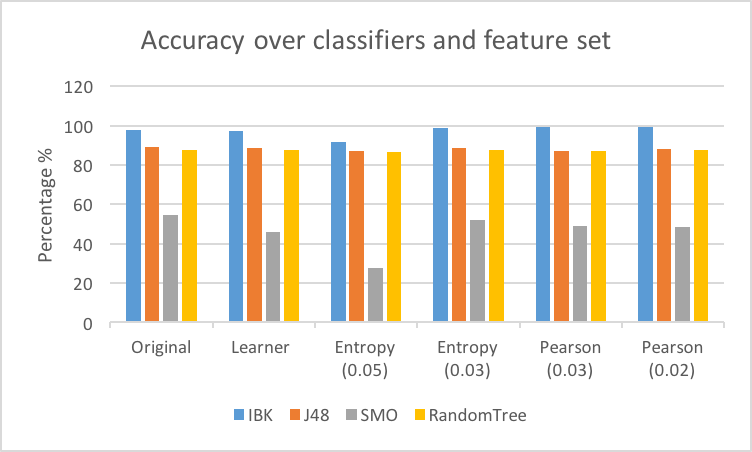
\includegraphics[scale=.65]{accuracy_p1}
 \caption{Accuracy for each dataset and classifiers for P1 datasets}
\label{figure2}
\end{figure}
\\\textbf{J48 Analysis}\\
It was found that the initialization of all J48 trees for each feature subset was identical. That is, each set of attributes derived the same root node and first layer of their J48 classifier. However, to emphasize the differences between the feature set trees, Figures 5 through 10 depict the general structures of each.
\begin{figure}[h]
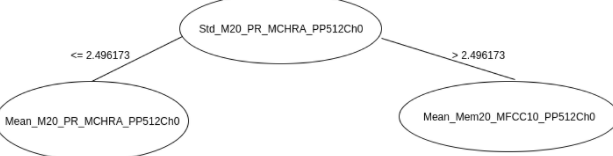
\includegraphics[scale=.35]{treenotes}
 \caption{Root Node and First layer for all P1 instances}
\label{figure3}
\end{figure}

The confusion matrix of each feature set was reviewed. The intersection of notes with the highest misclassified percentage value is summarized in Table \ref{table4}.

\begin{table}[h]
 \begin{center}
  \caption{P1 Feature subset highest confusion results}
\begin{tabular}{|C{2cm}|C{2cm}|C{2cm}|}
      \hline
          Filter (Threshold)& Intersection& Notes \\
         \hline
         Original & (m28, m27)  & 55 / 3420\\
         \hline
         Learner  & (m28, m27)  & 66 / 3420\\
          \hline
         Entropy (0.05) & (m23, m24) &73 / 3074\\
         \hline
         Entropy (0.03)  & (m28, m27)  & 75 / 3420\\
         \hline
         Pearson (0.03) & (m22, m21) & 72 / 3370\\
         \hline
         Pearson (0.02)  & (m28, m27)  & 61 / 3420\\
       \hline
\end{tabular}
\end{center}
 \label{table4}
\end{table}
It is not surprising that the feature sets have similar misclassified note intersections. It is reasonable to expect that similar sounding notes would be consistently misclassified no matter which subset and classifier were used. 


\subsection{P2 Dataset}
TBD...

\subsection{P3 Dataset}
TBD...
\subsection{P4 Dataset}
TBD...
\subsection{Exact Match Accuracy Comparison for PN Dataset}
TBD...
\section{Conclusion}\label{sec:Conclusion}
TBD...
\section{Future Work}
TBD...
% For bibtex users:
\bibliography{ISMIRtemplate}

% For non bibtex users:
%\begin{thebibliography}{citations}
%
%\bibitem {Author:00}
%E. Author.
%``The Title of the Conference Paper,''
%{\it Proceedings of the International Symposium
%on Music Information Retrieval}, pp.~000--111, 2000.
%
%\bibitem{Someone:10}
%A. Someone, B. Someone, and C. Someone.
%``The Title of the Journal Paper,''
%{\it Journal of New Music Research},
%Vol.~A, No.~B, pp.~111--222, 2010.
%
%\bibitem{Someone:04} X. Someone and Y. Someone. {\it Title of the Book},
%    Editorial Acme, Porto, 2012.
%
%\end{thebibliography}

\end{document}
